% Engine Numerical Loss Re-Rolls but Does Not Degrade -- LaTeX version of stage40-paper.md (draft).
% Build: run pdflatex twice. Needs a TeX Live with Korean support (the kotex package, collection-langkorean).
% XeLaTeX and LuaLaTeX also work: kotex loads the Korean support that matches the engine.
\documentclass[11pt]{article}

\usepackage{iftex}
\ifPDFTeX
  \usepackage[T1]{fontenc}
  \usepackage{lmodern}
\fi
\usepackage{kotex}
\usepackage[a4paper,margin=25mm]{geometry}
\usepackage{amsmath,amssymb}
\usepackage{booktabs,tabularx,array}
\usepackage{enumitem}
\usepackage[font=small,labelfont=bf]{caption}
\usepackage{tikz}
\usetikzlibrary{arrows.meta}
\usepackage[round]{natbib}
\usepackage{xcolor}
\usepackage[colorlinks=true,linkcolor=blue!50!black,citecolor=blue!50!black,urlcolor=blue!50!black]{hyperref}
\hypersetup{pdftitle={Engine Numerical Loss Re-Rolls but Does Not Degrade: An Exact-Baseline Study of LLM Failure Symptoms},
            pdfauthor={WooSungHyeun}}

\setlist{itemsep=2pt,topsep=4pt}
\newcolumntype{Y}{>{\raggedright\arraybackslash}X}
\def\bibpreamble{\emph{[Draft: entries to be completed and checked.]}\par\medskip}

\title{Engine Numerical Loss Re-Rolls but Does Not Degrade:\\
       An Exact-Baseline Study of LLM Failure Symptoms}
\author{WooSungHyeun\\[2pt]
        {\normalsize Chungwoon University, Republic of Korea}}
\date{{\normalsize Draft for arXiv (cs.CL / cs.LG), October 2026}\\[6pt]
      {\small Engine and experiments: \url{https://github.com/wwoosshh/GeulPU}\\
       Language and compiler: \url{https://github.com/wwoosshh/geul-lang}}}

\begin{document}
\maketitle

\begin{abstract}
Large language models sometimes produce familiar failures: endless repetition, text in an unrelated script, broken spelling,
wrong answers. One hypothesis attributes part of these failures to the numerical loss of inference engines---activations
re-quantized to 8~bits, half-precision attention and caches, reduction orders that change with the batch. Testing it requires
separating two effects that look alike in aggregate: loss that merely \emph{re-rolls} near-tie decisions, and loss that
systematically \emph{tilts} the model toward abnormal tokens. We use GeulPU---an inference engine whose arithmetic follows a
written precision contract, is bit-identical to a CPU reference, and produces identical bits across GPU generations and
vendors---as an exact, noise-free baseline, and compare it with llama.cpp and with a single-loss variant on
Qwen2.5-7B-Instruct and DeepSeek-R1-Distill-Qwen-7B (Q8\_0, greedy decoding, identical token inputs). On 696 Korean prompts
and 600 math problems, llama.cpp changes 89--100\% of the outputs, yet failures appear as often as they disappear (text in
another script: 36 new vs.\ 35 gone; wrong answers: 25 vs.\ 28). At 10,817 fragile steps---where an abnormal token competes
closely with the chosen one---we find no tilt toward other-script or byte-split tokens and a small tilt toward repetition
($+0.0039$~nat, about 0.4\% in odds) that is specific to repeating tokens. Under exact computation the model itself produces
most failures (32\% of long-form Korean answers loop to the length limit) and amplifies single slips: one forced other-script
token is followed by more other-script text in 80\% of continuations, against 34\% without it. All hypotheses, statistics
and decision rules were pre-registered.
\end{abstract}

% ---------------------------------------------------------------------------------------------------------------
\section{Introduction}\label{sec:intro}

Users of large language models (LLMs) know a small set of recurring failures: the model repeats a phrase until it runs out
of tokens, switches to an unrelated language or script in the middle of an answer, misspells a word it wrote correctly a
moment ago, or loses the point of a problem. These failures are usually attributed to the model---its training data, its
size, the decoding settings. A competing hypothesis is that part of them comes from the arithmetic of the inference engine.
Production engines trade precision for speed in many places: llama.cpp re-quantizes activations to 8~bits before its
quantized matrix multiplications, computes attention and stores the key--value cache in half precision, and, like most
engines, changes the order of floating-point reductions with the batch composition. Each of these choices perturbs the
logits slightly, and a slightly different logit at a near-tie can send a generation down a different path.

That engine numerics change outputs is well established. Changing the batch size, the number of GPUs or the engine alone
moves benchmark scores by several points \citep{yuan2025,pape2026}, prefix caching makes the same request diverge
\citep{patodiya2026}, and deterministic modes have been built to remove the variation on one machine \citep{he2025,qin2026}.
What is not established is whether this variation \emph{degrades} the output---produces more failures---or only
\emph{re-rolls} it, turning some answers worse and as many better. The two are indistinguishable in a single run; they
differ in the balance of failures that appear and disappear, and, at the level of single decisions, in whether the
perturbation is biased toward abnormal tokens.

Measuring that bias needs a baseline without engine noise. If the reference itself is noisy, selecting the decisions where
an abnormal token is close to the chosen one already depends on the noise, and the measured shift regresses toward zero. We
therefore use as the baseline an engine whose loss is limited to what a written contract specifies and whose bits do not
depend on batch, path, GPU or vendor (Section~\ref{sec:instrument}), feed identical token ids to every engine, and
pre-register the analysis.

Our contributions are:
\begin{enumerate}
\item A paired design with an exact baseline that separates \emph{re-rolling} (symptoms appear and disappear in equal
      numbers) from \emph{tilting} (a systematic shift toward abnormal tokens), with two pre-registered primary tests:
      trajectory-level McNemar tests and a step-level tilt test at fragile steps.
\item Evidence, for two 7B models at Q8\_0, that llama.cpp's numerical loss re-rolls but does not increase failures, and
      that its only detectable tilt is toward repetition and is about 0.4\% in odds.
\item Model-level measurements under exact computation: high failure base rates, self-amplification of a single
      other-script slip, no effect of a single injected anomaly in the previous turn, and the fraction of Korean syllables
      that are emitted as byte pieces.
\item The instrument itself: an open inference engine with a written precision contract whose outputs are bit-identical
      across NVIDIA generations, AMD and Intel GPUs and a CPU reference (Section~\ref{sec:instrument},
      Appendix~\ref{app:bitid}).
\end{enumerate}

% ---------------------------------------------------------------------------------------------------------------
\section{Related work}\label{sec:related}

\paragraph{Engine nondeterminism and evaluation.}
\citet{he2025} trace run-to-run differences in served LLMs to batch-dependent kernels and provide batch-invariant kernels;
vLLM and SGLang ship deterministic modes based on them. Vosti specifies deterministic inference formally and verifies an
engine against the specification, showing that the production modes still diverge under some execution variations
\citep{qin2026}. \citet{yuan2025} report accuracy swings of up to 9\% for DeepSeek-R1-Distill-Qwen-7B across GPU counts,
GPU types and batch sizes in bfloat16; \citet{pape2026} find that the choice of engine alone moves benchmark scores by up
to 16.6 points; \citet{patodiya2026} shows that llama.cpp's prefix cache makes repeated requests diverge, more so at
4~bits. These works establish variance; we ask whether the variance is biased.

\paragraph{Bit-exact inference across hardware.}
A CPU emulator can predict the bits of unmodified vLLM and Transformers runs on several NVIDIA GPUs, enabling verification
without changing the engine \citep{bitexact2026}. Fixed-shape reduction orders make linear layers identical across NVIDIA
Ampere, Ada and Hopper \citep{cooper2026}. Power-of-two weight scales make CUTLASS and Triton agree bitwise and expose the
limits of tolerance-based conformance tests \citep{chen2026}. Gensyn's REE reproduces inference across NVIDIA GPUs, Apple
GPUs and CPUs with a proprietary operator library. To our knowledge no published system shows identical bits across NVIDIA
and AMD GPUs with an open, written precision contract; we use such a system as an instrument rather than as the subject.

\paragraph{Failure modes.}
The Language Confusion Benchmark measures how often models answer in the wrong language \citep{marchisio2024a};
quantization hurts non-Latin scripts most, and automatic metrics understate the harm \citep{marchisio2024b}. Repetition is
self-reinforcing---each repetition makes the next more likely \citep{xu2022}---and repetition requests can make production
models diverge \citep{nasr2023}. Under-trained ``glitch'' tokens trigger anomalous behaviour \citep{land2024}. We are not
aware of work that injects or removes individual sources of numerical loss and measures their effect on these failures
with an exact baseline.

% ---------------------------------------------------------------------------------------------------------------
\section{The instrument: GeulPU and the geul language}\label{sec:instrument}

Our conclusions rest on two properties of the baseline: it is a complete inference engine that runs the same quantized model
files as llama.cpp on the same GPU, and its arithmetic is exact with respect to a written contract. Both are unusual for
software that is not built on Python, PyTorch or the CUDA toolkit, and the language it is written in is little known. This
section describes the stack from the bottom up; every number is taken from the two public repositories.

\subsection{The geul language and its compiler}\label{sec:geul}

geul (글, ``writing'') is a systems programming language whose grammar follows Korean: verbs come last, and the role of
each argument is marked by a case particle instead of its position. A function is declared with its roles,
\texttt{[문자열 원본을 문자열 대상에 복사]} (``copy a string \emph{source} to a string \emph{destination}''), and called by
role, \texttt{원본을 대상에 복사하다.}; the particles 을/를 (object), 에 (destination), 에서 (source), 로 (means) and
와/과 (companion) bind the arguments, and a call whose same-typed arguments carry no particle is a compile error. Types are
ordinary---정수 is a 64-bit integer, 짧은실수 a 32-bit float, \texttt{T 참조} a pointer---and memory is managed by hand.

The compiler is self-hosted: it is written in geul (about 10,000 lines) and compiles itself. A separate reference
implementation in Python (about 7,000 lines) is kept as the bootstrap seed and as a second implementation; the build checks
a fixpoint---the self-hosted compiler built by the reference implementation, then by itself, then by that output, is
byte-identical each time. Users need neither: the released compiler \texttt{geulc.exe} (geul 1.3.1, October 2026, MIT
license; a 182\,KB zip, also packaged for Windows as the PyPI package \texttt{geul}) builds everything described below. The
compiler has its own complete back end---lexer, parser, semantic analysis, a typed intermediate representation, an inliner,
an x86-64 code generator with linear-scan register allocation, a hand-written instruction encoder and PE32+/ELF64
writers---and uses no C compiler, assembler, linker or LLVM. A Windows executable it produces imports only
\texttt{kernel32.dll} (and \texttt{shell32.dll} for the command line); the Linux target (on the research branch) needs only
\texttt{libc.so.6}. Builds are reproducible byte for byte.

\subsection{From geul source to GPU instructions}\label{sec:backends}

GPU support lives on a research branch of the compiler. A GPU kernel is an ordinary geul function; GPU features are reached
through declared intrinsics: thread and block indices, shared memory, barriers, warp shuffles, asynchronous copies
(\texttt{cp.async}), integer tensor-core matrix multiply--accumulate (\texttt{mma.sync}\,\dots\,\texttt{m16n8k32}\,\dots\,%
\texttt{s8.s8.s32} and \texttt{m16n8k16}), \texttt{dp4a}, and fused multiply--add, which is emitted only where the source
writes it. Two back ends, both written in geul on top of the self-hosted front end, translate such kernels:

\begin{itemize}
\item \textbf{PTX back end} (2,574 lines)---emits PTX, NVIDIA's documented virtual instruction set. Every floating-point
      operation carries an explicit rounding mode (\texttt{.rn}), so the driver cannot fuse a multiply and an add on its
      own; approximate instructions and floating-point tensor cores, whose summation rounding the PTX specification leaves
      open, are not used.
\item \textbf{SPIR-V back end} (4,006 lines)---emits SPIR-V 1.6 compute shaders for Vulkan (AMD, Intel and NVIDIA). Kernel
      parameters become push constants and global memory becomes 64-bit device addresses; division and square root are
      written out to be correctly rounded, integer matrix products use cooperative-matrix instructions where the device
      offers them and subgroup operations otherwise.
\end{itemize}

\begin{figure}[t]
\centering
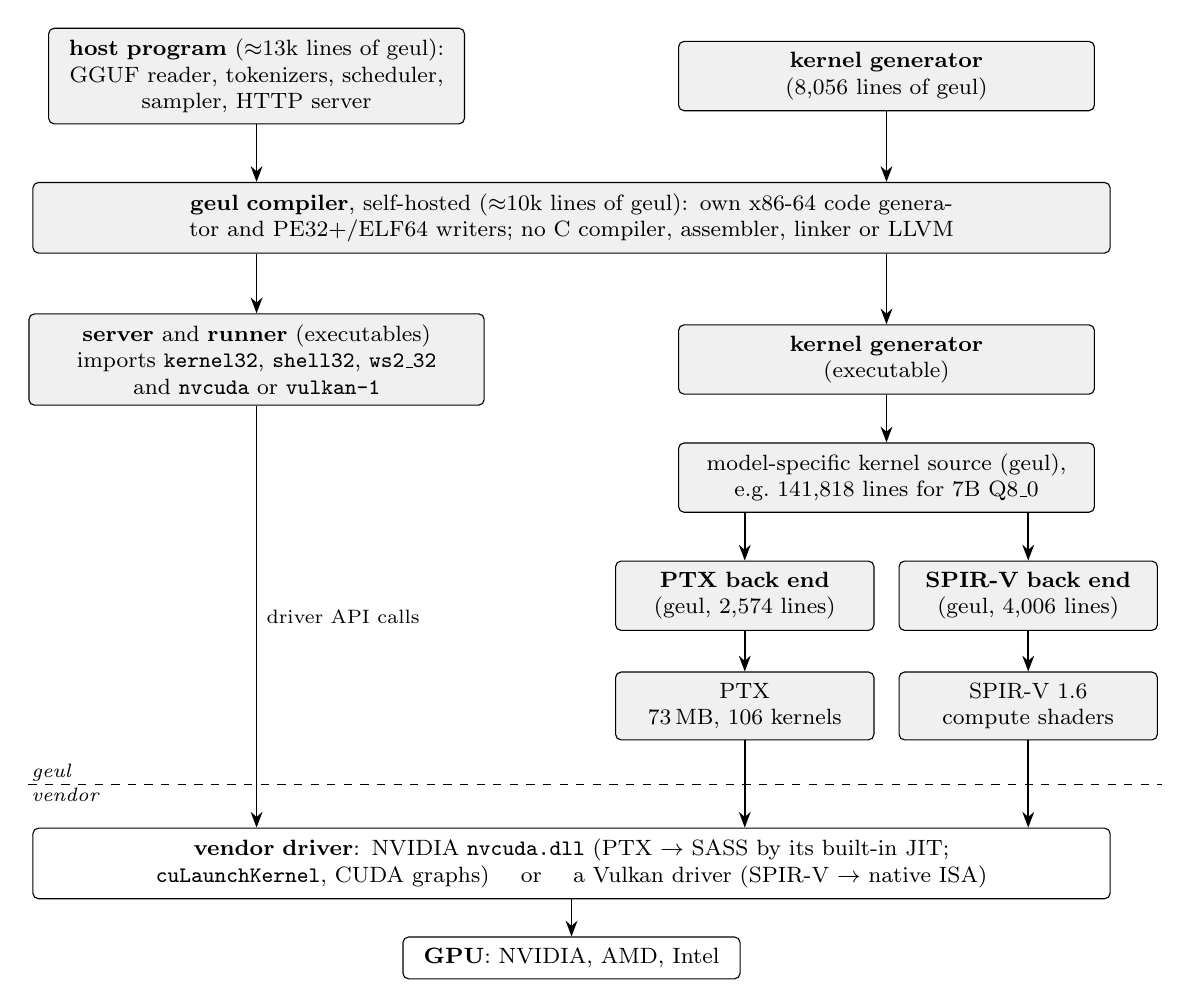
\begin{tikzpicture}[
    font=\footnotesize,
    >={Stealth[length=2mm]},
    geul/.style={draw, rounded corners=2pt, fill=black!6, align=center, inner sep=4pt},
    vendor/.style={draw, rounded corners=2pt, fill=white, align=center, inner sep=4pt},
    arr/.style={->, semithick},
  ]
  \node[geul, text width=5.0cm] (host) at (3.0,0)
    {\textbf{host program} ($\approx$13k lines of geul):\\GGUF reader, tokenizers, scheduler,\\sampler, HTTP server};
  \node[geul, text width=5.0cm] (gen) at (11.0,0)
    {\textbf{kernel generator}\\(8,056 lines of geul)};
  \node[geul, text width=13.4cm] (cc) at (7.0,-1.8)
    {\textbf{geul compiler}, self-hosted ($\approx$10k lines of geul): own x86-64 code generator and PE32+/ELF64 writers;
     no C compiler, assembler, linker or LLVM};
  \node[geul, text width=5.5cm] (srv) at (3.0,-3.6)
    {\textbf{server} and \textbf{runner} (executables)\\imports \texttt{kernel32}, \texttt{shell32}, \texttt{ws2\_32}\\
     and \texttt{nvcuda} or \texttt{vulkan-1}};
  \node[geul, text width=5.0cm] (kg) at (11.0,-3.6)
    {\textbf{kernel generator}\\(executable)};
  \node[geul, text width=5.0cm] (ks) at (11.0,-5.1)
    {model-specific kernel source (geul),\\e.g.\ 141,818 lines for 7B Q8\_0};
  \node[geul, text width=3.0cm] (pb) at (9.2,-6.6)
    {\textbf{PTX back end}\\(geul, 2,574 lines)};
  \node[geul, text width=3.0cm] (sb) at (12.8,-6.6)
    {\textbf{SPIR-V back end}\\(geul, 4,006 lines)};
  \node[geul, text width=3.0cm] (ptx) at (9.2,-8.0)
    {PTX\\73\,MB, 106 kernels};
  \node[geul, text width=3.0cm] (spv) at (12.8,-8.0)
    {SPIR-V 1.6\\compute shaders};
  \draw[dashed] (0.1,-9.0) -- (14.5,-9.0);
  \node[anchor=south west, font=\scriptsize\itshape, inner sep=1pt] at (0.1,-9.0) {geul};
  \node[anchor=north west, font=\scriptsize\itshape, inner sep=1pt] at (0.1,-9.0) {vendor};
  \node[vendor, text width=13.4cm] (drv) at (7.0,-10.0)
    {\textbf{vendor driver}: NVIDIA \texttt{nvcuda.dll} (PTX $\to$ SASS by its built-in JIT; \texttt{cuLaunchKernel},
     CUDA graphs) \quad or \quad a Vulkan driver (SPIR-V $\to$ native ISA)};
  \node[vendor, text width=4.0cm] (gpu) at (7.0,-11.2)
    {\textbf{GPU}: NVIDIA, AMD, Intel};
  \draw[arr] (host.south) -- (host.south |- cc.north);
  \draw[arr] (gen.south) -- (gen.south |- cc.north);
  \draw[arr] (cc.south -| srv.north) -- (srv.north);
  \draw[arr] (cc.south -| kg.north) -- (kg.north);
  \draw[arr] (kg) -- (ks);
  \draw[arr] (ks.south -| pb.north) -- (pb.north);
  \draw[arr] (ks.south -| sb.north) -- (sb.north);
  \draw[arr] (pb) -- (ptx);
  \draw[arr] (sb) -- (spv);
  \draw[arr] (ptx.south) -- (ptx.south |- drv.north);
  \draw[arr] (spv.south) -- (spv.south |- drv.north);
  \draw[arr] (srv.south) -- (srv.south |- drv.north) node[midway, right, font=\scriptsize] {driver API calls};
  \draw[arr] (drv) -- (gpu);
\end{tikzpicture}
\caption{The GeulPU stack. Everything above the dashed line is written in geul and compiled by the geul compiler; below it
is the GPU vendor's driver.}
\label{fig:stack}
\end{figure}

At run time the engine hands PTX text to the NVIDIA driver (\texttt{cuModuleLoadData}), whose built-in just-in-time compiler
translates it to the GPU's native machine code (SASS), and launches kernels with \texttt{cuLaunchKernel} and CUDA graphs
(Figure~\ref{fig:stack}). On Vulkan it creates shader modules and compute pipelines and records dispatches; a thin layer maps
the driver-API calls the engine uses onto Vulkan, so the engine code is shared. Nothing from the CUDA toolkit---\texttt{nvcc},
\texttt{ptxas}, \texttt{cudart}, cuBLAS---or from a Vulkan SDK is used to build or run the engine; the
continuous-integration job installs \texttt{ptxas} only to check register spills. This is the same layer at which other
engines meet the GPU: llama.cpp ships kernels compiled ahead of time with \texttt{nvcc} and calls cuBLAS, vLLM runs PyTorch,
CUDA and Triton kernels; GeulPU generates its own kernels and talks only to the driver. The vendors' closed compilers below
PTX and SPIR-V are outside the contract, which is why bit-identity across devices is established empirically
(Appendix~\ref{app:bitid}) rather than proved.

\subsection{The kernel generator and the engine}\label{sec:engine}

A kernel generator, itself a geul program (8,056 lines), writes the kernel source specialized to a model's shape and weight
format. For Qwen2.5-7B at Q8\_0 it writes 141,818 lines of geul, which the PTX back end turns into 73\,MB of PTX holding 106
kernels and 6,488 tensor-core instructions; the module is built on the user's machine on first use, and the CI regenerates
18 such modules and compares their SHA-256 hashes with the recorded ones.

The host---about 13,000 lines of geul (15,000 with its test programs)---is a complete serving engine:
\begin{itemize}
\item \textbf{Models}: reads GGUF files with Q8\_0, Q4\_0, Q4\_K, Q5\_K and Q6\_K weights (including the Q4\_K\_M and
      Q5\_K\_M mixes); architectures qwen2, qwen3 and llama---Qwen2.5, Qwen3, DeepSeek-R1-Distill-Qwen, Llama~3.1 and 3.2,
      Mistral v0.3---with head size 128 (Qwen2.5-0.5B only through the command-line runner).
\item \textbf{Text}: byte-level BPE with Unicode NFC, the Llama~3 BPE and SentencePiece tokenizers, written in geul, which
      match llama.cpp token for token on 2,000 lines of test text; chat templates checked against the GGUF's Jinja
      templates.
\item \textbf{Serving}: an OpenAI-compatible HTTP server (chat and text completions, streaming, \texttt{/tokenize}), up to 8
      slots with continuous batching and per-slot prompt reuse, a decode step captured as one CUDA graph, sampling and
      log-probabilities computed under the same written contract.
\item \textbf{Footprint}: the CUDA server imports only \texttt{kernel32}, \texttt{shell32}, \texttt{ws2\_32} and
      \texttt{nvcuda} (43 driver-API functions); the Vulkan server imports \texttt{vulkan-1} (48 functions) instead of
      \texttt{nvcuda}. The CI checks these import tables.
\end{itemize}

On an RTX 4070 Ti, its decoding speed is within $\pm5$\% of llama.cpp for Qwen2.5-7B and Llama-3.1-8B at Q8\_0 and
Q4\_K\_M (0.97--1.05$\times$ the time per token, depending on the llama.cpp build and the context length); prompt
processing is faster than llama.cpp below about 128 tokens and up to 1.3--1.4$\times$ (Q8\_0) and 1.4--1.6$\times$ (k-quant
formats) slower at 8,192 tokens. Not everything is in geul: the CPU reference of the contract, the test harnesses and the
benchmarks are Python (NumPy), and the optional desktop app's interface is JavaScript. The engine is Windows-first (Linux
builds were tested under WSL2), uses one GPU, and needs compute capability 8.0 or newer on the CUDA path.

\subsection{The precision contract}\label{sec:contract}

GeulPU's arithmetic follows a written contract (\texttt{docs/contract.md}) that leaves the hardware no discretion:
\begin{itemize}
\item \textbf{Linear layers.} Each block of 32 activations is scaled by a power of two from its largest value and rounded to
      integers of at most $2^{14}$, stored as two signed 8-bit digits. The products with the model's integer weights are
      summed exactly on int8 tensor cores (prompts) or with \texttt{dp4a} (decoding)---exact integer sums do not depend on
      summation order---then rounded once per block and accumulated with fused multiply--adds in a fixed order.
\item \textbf{Attention.} Queries, keys and values are converted the same way and the key--value cache stores the digits;
      scores are exact integer sums rounded once; the exponential is a written polynomial; keys are processed in fixed
      64-key chunks and folded in a fixed two-level order.
\item \textbf{Everything else.} Normalizations use fixed reduction trees, rotary tables are correctly rounded, and one rule
      fixes how subnormal numbers flush on every path (PTX \texttt{.ftz}, the Vulkan drivers and the CPU reference agree on
      it); sampling and log-probabilities are computed in float64 in a fixed order.
\end{itemize}

Because nothing depends on how the work is split, the bits do not depend on batch, slot, chunking, prompt-versus-decode path,
GPU or vendor, and they equal those of a CPU reference implementation of the contract in NumPy; this is checked on kernel
test cases, on whole models end to end, and across machines (Appendix~\ref{app:bitid}). The contract is close to exact: on
Qwen2.5-0.5B (Q8\_0) the Kullback--Leibler divergence of its next-token distributions from an fp64 computation is
$2.24\times10^{-6}$, against $1.38\times10^{-3}$ for llama.cpp; for 7B and 14B the corresponding ratios (1/3,805 and
1/4,467) come from a simulation of the rounding points rather than from the engine. Exactness has a price: at equal
optimization, keeping two activation digits instead of one makes prompt processing 1.26--1.38$\times$ slower (a lower bound
measured by switching the tile kernels), while decoding, which is memory-bound, is unaffected.

% ---------------------------------------------------------------------------------------------------------------
\section{Method}\label{sec:method}

\subsection{Arms and inputs}\label{sec:arms}

\begin{itemize}
\item \textbf{G (exact baseline)}---GeulPU under its precision contract (Section~\ref{sec:instrument}): loss only where the
      contract writes it, no dependence on batch, slot or execution path. OpenAI-compatible server, 8 slots.
\item \textbf{L (production engine)}---llama.cpp build b11669 (Windows CUDA 13.4), \texttt{llama-server} with default
      settings (flash attention \emph{auto}, F16 key--value cache, prompt cache on), 8 parallel slots, the same GGUF files.
\item \textbf{V (one loss)}---G with a single change: the input activations of all linear layers rounded to one digit
      instead of two (block grid $2^{E-5}$, $|n|\le 64$---the same class as llama.cpp's 8-bit activation
      re-quantization); attention and everything else unchanged.
\end{itemize}

All prompts were rendered once with llama.cpp's \texttt{/apply-template} (the chat template stored in the GGUF) and tokenized
with \texttt{/tokenize}; every arm received the same token ids. Decoding was greedy (temperature 0) with the same maximum
length and end tokens, so the arms differ only in arithmetic. The context was 4,096 tokens per slot. Models:
Qwen2.5-7B-Instruct (Korean prompts) and DeepSeek-R1-Distill-Qwen-7B (math; R1-Distill below), both Q8\_0, so the weight loss
is identical across arms and small.

\subsection{Prompt sets}\label{sec:sets}

Table~\ref{tab:sets} lists the prompt sets: natural prompts, and trigger sets built to make each symptom frequent enough to
study.

\begin{table}[t]
\centering
\small
\caption{Prompt sets.}
\label{tab:sets}
\begin{tabularx}{\textwidth}{@{}l r r l Y@{}}
\toprule
Set & Items & Max new & Model & Source \\
\midrule
Natural: LCB Korean & 396 & 1,024 & Qwen2.5 & Language Confusion Benchmark \citep{marchisio2024a}, Korean native and
  cross-lingual prompts (Apache-2.0); 3 overlong prompts excluded \\
Natural: long-form Korean & 300 & 2,048 & Qwen2.5 & 60 topics $\times$ 5 forms (``write 2,000 characters or more'') \\
Natural: math & 600 & 3,200 & R1-Distill & gsm8k test \citep{cobbe2021}, first 600, with ``Please reason step by step,
  and put your final answer within \texttt{\textbackslash boxed\{\}}.'' \\
Trigger: rare syllables & 200 & 512 & Qwen2.5 & ``Copy the following text exactly'': 80--200-character texts with $\geq 6$
  syllables that the tokenizer splits into byte pieces \\
Trigger: mixed script & 200 & 1,024 & Qwen2.5 & Korean questions about Chinese/Japanese words and names written in their
  own script \\
Trigger: repetition & 200 & 2,048 & Qwen2.5 & requests to repeat a word or sentence, count in Korean words, continue a
  pattern \\
Contamination dialogs & $100\times4$ & 512 + 1,024 & Qwen2.5 & two-turn dialogs; the first answer is G's own, unchanged or
  with one injected anomaly \\
\bottomrule
\end{tabularx}
\end{table}

\subsection{Symptoms}\label{sec:symptoms}

All symptoms are decided automatically from token ids and text:
\begin{itemize}
\item \textbf{S1 endless repetition}---the generation hit the length limit and its tail is an exact repetition: the
      smallest period $p\le 512$ tokens whose repetition covers at least $\max(3p, 64)$ final tokens.
\item \textbf{S2 other-script text} (Korean sets)---S2a: a run of two or more letters that are neither Hangul nor Latin
      (Han, kana, Cyrillic, Thai, Arabic, Devanagari, \dots; Greek excluded), outside code, not present in the question;
      or S2b: less than 50\% of the letters are Hangul.
\item \textbf{S3 unfinished / S4 wrong answer} (math)---S3: length limit without \texttt{\textbackslash boxed\{\}}; S4: the
      last boxed number differs from the gold answer (S3 counts as wrong).
\item \textbf{S6 broken spelling} (copy trigger)---the copied span differs from the source by at least one character, or
      contains a broken UTF-8 character.
\end{itemize}

\subsection{Fragile steps and tilt}\label{sec:tilt}

At each generated step of G, let $a$ be the chosen token (greedy: G's top-1) and $b$ the highest-ranked abnormal candidate
of a given type among G's top 20:
\begin{itemize}
\item \textbf{O (other script)}---$a$ is Hangul, Latin, digit or symbol; $b$ contains a letter of another script
      (byte-piece tokens are classified by the script their lead byte implies);
\item \textbf{R (repetition)}---appending $a$ does not copy an earlier 8-token sequence of the answer, appending $b$ does;
\item \textbf{C (byte-split character)}---the step is inside a multi-byte character (earlier tokens left the UTF-8 sequence
      incomplete), and $b$ completes a different character or breaks the encoding.
\end{itemize}
A step is \emph{fragile} if the margin $m = \ln p_G(a) - \ln p_G(b)$ is below $\ln 10$. For an arm $X\in\{L,V\}$, the tilt
at the step is
\begin{equation}\label{eq:tilt}
  \Delta_X = \bigl[\ln p_X(b) - \ln p_X(a)\bigr] - \bigl[\ln p_G(b) - \ln p_G(a)\bigr],
\end{equation}
computed on the same prefix (G's answer). Zero-mean numerical noise gives $\mathbb{E}[\Delta]=0$; a systematic shift toward
abnormal tokens gives $\Delta>0$. As a control we compute the same quantity for the highest-ranked \emph{normal} alternative
at the same step. The mean $\Delta$ is estimated over all fragile steps with a 95\% interval from a bootstrap that resamples
prompts (10,000 resamples, seed 40); the three types are corrected with Holm's method. Decision labels (pre-registered):
\emph{tilts toward abnormal} (mean $>0$, corrected $p<0.05$), \emph{tilts away}, \emph{no tilt} (corrected $p\ge 0.05$ and
the interval within $\pm0.05$~nat), \emph{undecided} otherwise or with fewer than 200 steps.

To obtain L's distribution at G's prefixes we drive llama.cpp through its C API: the prompt is evaluated in one batch, as the
server does, and G's answer tokens are then fed one at a time, eight sequences per batch, which is the server's generation
path. We validated this against \texttt{llama-server} itself (Section~\ref{sec:validity}).

\subsection{Trajectories, propagation and contamination}\label{sec:traj-method}

\begin{itemize}
\item \textbf{Trajectories (primary).} For each prompt, a symptom present only in the arm is \emph{new}, present only in G
      \emph{gone}. H1: Qwen2.5-7B, natural Korean sets, S2. H2: R1-Distill, math, S4. Exact McNemar tests, Holm over the
      two. Labels: \emph{increases}, \emph{decreases}, \emph{shakes but does not increase} (new + gone $\ge 40$, corrected
      $p\ge 0.05$), \emph{undecided} (new + gone $<40$; H2 would first add the next 600 problems once---not needed).
\item \textbf{Propagation.} At up to 100 fragile steps per type (seed 40) we force $b$ in G and continue for 256 tokens, and
      compare with G's own continuation after $a$: does a symptom of the same type appear again?
\item \textbf{Contamination.} We insert one anomaly into G's first answer of a two-turn dialog---a Chinese word, a
      misspelled word, or a duplicated sentence---and compare the second answer with the one generated after the unchanged
      first answer.
\end{itemize}

\subsection{Pre-registration}\label{sec:prereg}

The design, the statistics and the decision rules were committed before any measurement (commit \texttt{9190f76}); the prompt
sets and tools before the main runs (\texttt{d88b6cf}, \texttt{eedb304}); deviations are listed in Appendix~\ref{app:dev}.

% ---------------------------------------------------------------------------------------------------------------
\section{Results}\label{sec:results}

\subsection{Validity checks}\label{sec:validity}

\begin{itemize}
\item \textbf{Identical inputs}: in every arm and item, the number of prompt tokens the engine received equals the number
      sent.
\item \textbf{Determinism}: 50 prompts re-run at concurrency 1 give identical tokens in G and in V; 50 forced-token
      continuations re-run give identical tokens.
\item \textbf{The L measurement path}: for 50 prompts generated by \texttt{llama-server} with one slot, the follower's argmax
      equals the server's token at all 3,358 steps up to the first divergence from G.
\item \textbf{Human check of the symptom judges} (20 items per symptom: 10 judged positive, 10 negative): repetition 19/20,
      other-script 17/20---below the pre-registered 90\%. The other-script judge counted Han characters used to explain a
      Chinese word and English song titles quoted from the prompt. Because both arms of each comparison use the same
      judge, the paired tests are not biased toward either arm; a stricter post-hoc judge (Section~\ref{sec:sensitivity})
      leaves every conclusion unchanged.
\end{itemize}

\subsection{Trajectories: re-rolled, not degraded}\label{sec:trajectories}

\begin{table}[t]
\centering
\small
\caption{Primary trajectory tests, llama.cpp (L) against the exact baseline (G). G / L: items with the symptom in each arm;
new: items with the symptom only in L; gone: only in G.}
\label{tab:traj}
\begin{tabularx}{\textwidth}{@{}Y r c r r r l@{}}
\toprule
Test & Items & G / L & New & Gone & Holm $p$ & Label \\
\midrule
H1: Qwen2.5-7B, natural Korean, other script (S2) & 696 & 94 / 95 & 36 & 35 & 1.0 &
  \begin{tabular}[t]{@{}l@{}}shakes but\\does not increase\end{tabular} \\
\addlinespace
H2: R1-Distill-7B, gsm8k, wrong answer (S4) & 600 & 80 / 77 & 25 & 28 & 1.0 &
  \begin{tabular}[t]{@{}l@{}}shakes but\\does not increase\end{tabular} \\
\bottomrule
\end{tabularx}
\end{table}

Table~\ref{tab:traj} gives the primary tests. llama.cpp produced a different text for 89\% of the LCB prompts, all 300
long-form prompts and 97\% of the math problems; the first divergence came after a median of 66, 57 and 138 tokens. The
single loss V changed even more (96--100\%, median first divergence 21--61 tokens) and was equally balanced (H1$'$: 48 new
vs.\ 43 gone; H2$'$: 25 vs.\ 28). No secondary comparison moved: endless repetition in long-form answers 19 new vs.\ 15
gone, broken copies 4 vs.\ 3, unfinished math 29 vs.\ 35 (all $p\ge 0.25$). Accuracy on the 600 math problems was 86.7\%
(G) and 87.2\% (L).

\subsection{Tilt: only toward repetition, and small}\label{sec:tilt-results}

\begin{table}[t]
\centering
\small
\caption{Tilt at fragile steps of Qwen2.5-7B (972,380 output tokens). $\bar{\Delta}$: mean tilt in nats
(Eq.~\ref{eq:tilt}); CI: 95\% prompt-cluster bootstrap interval; control: the same quantity for the best normal alternative
at the same steps; last row: steps at which llama.cpp itself chose $b$.}
\label{tab:tilt}
\begin{tabular}{@{}l lll@{}}
\toprule
 & O: other script & R: repetition & C: byte-split character \\
\midrule
Fragile steps & 3,042 & 4,975 & 2,800 \\
\quad per 1k tokens & 3.13 & 5.12 & 2.88 \\
\addlinespace
$\bar{\Delta}_L$ & $-0.00006$ & $\mathbf{+0.0039}$ & $-0.0034$ \\
\quad 95\% CI & $[-0.0046, +0.0046]$ & $\mathbf{[+0.0015, +0.0063]}$ & $[-0.0074, +0.0004]$ \\
\quad Holm $p$ & 0.99 & \textbf{0.003} & 0.18 \\
\quad Label & no tilt & \textbf{tilts toward abnormal} & no tilt \\
\quad Control $\bar{\Delta}_L$ & $+0.0010$ & $-0.0011$ & $+0.008$ (103 steps) \\
\addlinespace
$\bar{\Delta}_V$ & $-0.018$ & $+0.012$ & $+0.012$ \\
\quad 95\% CI & $[-0.031, -0.006]$ & $[+0.005, +0.018]$ & $[+0.002, +0.023]$ \\
\addlinespace
L chose $b$ & 37 (1.2\%) & 101 (2.0\%) & 55 (2.0\%) \\
\bottomrule
\end{tabular}
\end{table}

The repetition tilt (Table~\ref{tab:tilt}) corresponds to a 0.39\% increase in the odds of the repeating token; the control
at the same steps is zero, so the shift is specific to repeating tokens rather than a general flattening. llama.cpp chose the
abnormal token only where the margin was below 0.5~nat (below 0.25~nat: 36 of 206 O steps, 101 of 754 R steps, 52 of 314 C
steps). The single activation loss tilts about three times more toward repetition, also tilts toward byte errors (where
llama.cpp shows no tilt), and tilts \emph{away} from other-script tokens: different losses tilt in different directions. On
R1-Distill's English reasoning (8,121 repetition steps) neither L nor V tilts ($-0.0006$, $-0.0009$).

\subsection{Under exact computation, the model produces the failures}\label{sec:base-rates}

\begin{table}[t]
\centering
\small
\caption{Symptom counts of Qwen2.5-7B under exact computation (arm G).}
\label{tab:base}
\begin{tabular}{@{}l r r r r@{}}
\toprule
Set & Items & S1 repetition & S2 other script & S6 broken copy \\
\midrule
Natural: LCB Korean & 396 & 6 & 65 (16\%) & -- \\
Natural: long-form Korean & 300 & 95 (32\%) & 29 & -- \\
Trigger: rare syllables & 200 & 10 & 44 & 115 (58\%) \\
Trigger: mixed script & 200 & 6 & 80 (40\%)$^{a}$ & -- \\
Trigger: repetition & 200 & 52 (26\%) & 1 & -- \\
\bottomrule
\multicolumn{5}{@{}l}{\footnotesize $^{a}$ 36 (18\%) by the stricter judge of Section~\ref{sec:sensitivity}.}
\end{tabular}
\end{table}

R1-Distill answered 86.7\% of the math problems correctly; 59 of the 80 wrong answers did not finish within 3,200 tokens.
On the rare-syllable trigger the exact model sometimes loops on an emoji, or invents a Chinese ``user'' turn and repeats a
character until the limit (Table~\ref{tab:base}). In real Korean text 11.2\% (Qwen2.5) and 8.5\% (Llama~3.1) of syllables are
emitted across two or more byte-piece tokens; only 2,512 (Qwen2.5) and 599 (Llama~3.1) of the 11,172 Hangul syllables are
single tokens.

\subsection{Propagation and contamination}\label{sec:propagation}

Forcing the abnormal token at an other-script fragile step makes more other-script text appear within the next 256 tokens in
80 of 100 continuations, against 34 after the original token (47 vs.\ 1 discordant, $p=3.5\times10^{-13}$); 99 of the 100
forced tokens were complete characters, and excluding the first two characters of the continuation gives 77 of 99, so the
effect is not a mechanical completion of a byte sequence. For repetition and byte-split steps the measure saturated (the
original continuations already showed the symptom in 89\% and 97\% of cases). A single anomaly injected into the previous
answer did not raise symptoms in the next one: other-script text 32 vs.\ 37 (5 new, 10 gone), broken copies 53 vs.\ 54,
repeated sentences 7 vs.\ 10.

\subsection{Sensitivity to the symptom judge}\label{sec:sensitivity}

A stricter judge, defined after the human check and before re-computation, ignores foreign text inside quotes or brackets or
followed by a Hangul gloss, and ignores Latin words that occur in the prompt. It agrees with the human labels on 19 of 20
items (the items were used to design it, so this is not an independent check). All conclusions hold: H1 31 new vs.\ 31
gone, H1$'$ 41 vs.\ 43, propagation 78\% vs.\ 31\%. Only the rates move: the mixed-script trigger's other-script rate falls
from 40\% to 18\%; the LCB rate from 16\% to 15\%.

% ---------------------------------------------------------------------------------------------------------------
\section{Discussion}\label{sec:discussion}

\paragraph{Re-rolling, not tilting.}
At the precision of a mainstream engine with 8-bit weights, numerical loss behaves like re-sampling at near-ties: almost every
long answer changes, and the failures it creates are matched by failures it removes. The harm is reproducibility---the
symptom status of about one item in ten (71 of 696, 53 of 600) depends on the engine---not quality.

\paragraph{The one tilt.}
The repetition tilt is real and specific, and the single activation loss shows it three times more strongly, which points to
activation rounding as one contributor. At 0.4\% in odds it did not reach the trajectory level in our samples.

\paragraph{The model is the source.}
Under exact arithmetic the model loops on a third of long Korean answers, mixes scripts in a sixth of LCB answers and fails
most rare-syllable copies; once a single other-script token is emitted, the model continues in that script most of the time.
Mitigations for these failures belong to the model and the decoding procedure rather than to the arithmetic.

\paragraph{What an exact baseline is for.}
It made a 0.004-nat shift measurable and every case replayable bit for bit. The same result also bounds its practical value
for users: effects small enough to need an exact baseline are too small to change what users see.

\paragraph{Limitations.}
Two 7B models of one family at Q8\_0, greedy decoding, one production engine (llama.cpp) on one GPU (RTX 4070 Ti), mostly
Korean prompts, automatic judges (the other-script judge agreed with a human on 85\%), and only engine-level loss: we did not
test larger losses such as 4-bit key--value caches, longer contexts or sampling. Propagation could not be measured for
repetition and byte-split steps because the measure saturated. Closed frontier models could not be studied; the mechanisms
(byte pieces, near-ties, self-amplification) are generic, but their rates there are unknown.

% ---------------------------------------------------------------------------------------------------------------
\section{Conclusion}\label{sec:conclusion}

With an exact, noise-free baseline and identical inputs, the numerical loss of a production engine re-rolls LLM outputs
without increasing their familiar failures; its only measurable bias is a 0.4\% tilt toward repetition. The failures come
from the model, which also amplifies its own slips. Making inference arithmetic exact buys reproducibility, not fewer
failures, at this precision.

\section*{Acknowledgements and AI assistance}

\emph{[To be agreed with the author.]} The geul compiler, GeulPU and the experiment code were developed by the author with
substantial assistance from AI coding agents (Anthropic Claude), which also helped draft this manuscript. The author designed
the study, approved the pre-registration and checked the symptom judges by hand.

% ---------------------------------------------------------------------------------------------------------------
\begin{thebibliography}{14}

\bibitem[arXiv:2606.00279(2026)]{bitexact2026}
Bit-exact AI inference verification without performance tradeoffs. arXiv:2606.00279, 2026. [Authors to be added.]

\bibitem[Chen(2026)]{chen2026}
T.-R. Chen. Deterministic LLM inference across GPU kernels: power-of-two INT8 quantization scales and the limits of
tolerance-based conformance. arXiv:2609.00363, 2026.

\bibitem[Cobbe et~al.(2021)]{cobbe2021}
K.~Cobbe et~al. Training verifiers to solve math word problems. arXiv:2110.14168, 2021.

\bibitem[Cooper et~al.(2026)]{cooper2026}
L.~Cooper et~al. Accelerating the mitigation of LLM inference nondeterminism across GPU architectures. arXiv:2609.25624,
2026.

\bibitem[He et~al.(2025)]{he2025}
H.~He et~al. Defeating nondeterminism in LLM inference. Thinking Machines Lab, 2025.

\bibitem[Land and Bartolo(2024)]{land2024}
S.~Land and M.~Bartolo. Fishing for Magikarp: automatically detecting under-trained tokens in large language models.
arXiv:2405.05417, 2024.

\bibitem[Marchisio et~al.(2024a)]{marchisio2024a}
K.~Marchisio et~al. Understanding and mitigating language confusion in LLMs. arXiv:2406.20052, 2024a.

\bibitem[Marchisio et~al.(2024b)]{marchisio2024b}
K.~Marchisio et~al. How does quantization affect multilingual LLMs? arXiv:2407.03211, 2024b.

\bibitem[Nasr et~al.(2023)]{nasr2023}
M.~Nasr et~al. Scalable extraction of training data from (production) language models. arXiv:2311.17035, 2023.

\bibitem[Pape et~al.(2026)]{pape2026}
D.~Pape et~al. The silent hyperparameter: quantifying the impact of inference backends on LLM reproducibility.
arXiv:2605.19537, 2026.

\bibitem[Patodiya(2026)]{patodiya2026}
A.~Patodiya. Same request, different answer: quantization amplifies cache-induced divergence in LLM serving.
arXiv:2609.04748, 2026.

\bibitem[Qin et~al.(2026)]{qin2026}
J.~Qin et~al. Vosti: specifying, implementing and verifying deterministic LLM inference. arXiv:2609.38981, 2026.

\bibitem[Xu et~al.(2022)]{xu2022}
J.~Xu et~al. Learning to break the loop: analyzing and mitigating repetitions for neural text generation.
arXiv:2206.02369, 2022.

\bibitem[Yuan et~al.(2025)]{yuan2025}
J.~Yuan et~al. Give me FP32 or give me death? Challenges and solutions for reproducible reasoning. arXiv:2506.09501, 2025.

\end{thebibliography}

% ---------------------------------------------------------------------------------------------------------------
\appendix

\section{Bit-identity evidence for GeulPU}\label{app:bitid}

\paragraph{Within one machine.}
Against the CPU reference: every logit row of Qwen2.5-0.5B; 26,155,008 logits of Qwen2.5-7B Q8\_0 with zero differences;
106 kernel cases for Q4\_0 and 349 for the k-quants plus whole files; the Qwen3, Llama~3.x and Mistral files end to end.
Across execution paths: decode graph, whole prompt, prompt in four pieces, one row at a time and repeated runs give identical
logits and key--value caches; wikitext-2 log-likelihoods are bit-identical whether text is fed in chunks of 512, 128 or 1
token (llama.cpp's perplexity moves between 15.8171 and 15.8200 with its batch settings); the server returns identical
tokens and logit hashes for 4 models $\times$ 12 requests $\times$ 4 schedules (llama-server changed its greedy answer in 11
of 12 cases); lm-evaluation-harness item results are identical at 1 and 8 concurrent requests and on CUDA and Vulkan; Linux
(WSL2) output equals Windows output byte for byte.

\paragraph{Across machines.}
A cross-check package builds the compiler, the back ends, the server and the 7B module from source on a volunteer's PC (the
build hashes are compared with the reference), downloads DeepSeek-R1-Distill-Qwen-7B Q8\_0, solves 32 synthetic math
problems greedily ($\le$3,200 tokens) and compares the texts and a 64-bit FNV hash of the full 152,064-entry logit row at
every step (Table~\ref{tab:cross}).

\begin{table}[ht]
\centering
\small
\caption{Cross-machine check. Texts: problems whose text is identical to the reference; logit hashes: steps whose
logit-row hash is identical to the reference.}
\label{tab:cross}
\begin{tabularx}{\textwidth}{@{}l Y l r r@{}}
\toprule
PC & GPU (path) & Driver & Texts & Logit hashes \\
\midrule
Reference & NVIDIA RTX 4070 Ti, Ada (CUDA) & 616.56 & reference & reference \\
Volunteer 1 & NVIDIA RTX 5070, Blackwell (CUDA) & 596.21 & 32/32 & 82,673/82,673 \\
Volunteer 2 & NVIDIA RTX 3080 Ti, Ampere (CUDA) & 616.92 & 32/32 & 82,673/82,673 \\
Reference & RTX 4070 Ti (Vulkan; two kernel variants) & 616.56 & 32/32 & 82,673/82,673 \\
Volunteer 3 & AMD RX 9060 XT, RDNA4 (Vulkan; two variants) & AMD 26.8.1 & 32/32 & 82,673/82,673 \\
Volunteer 4 & AMD RX 9060 XT (Vulkan; two variants) & AMD 25.20.42.14 & 32/32 & 82,673/82,673 \\
\bottomrule
\end{tabularx}
\end{table}

The 82,673 hashed steps are 82,657 generated tokens plus the 16 end-of-sequence steps. On the same reference PC,
llama-server produced identical texts for 0 of the 32 problems between 1 and 8 concurrent requests and changed 6 final
answers. An Intel UHD 770 integrated GPU reproduced the 0.5B model's records (larger models exceed its memory limits). Each
run built the engine from the commit current at the time; later engine changes left the reference outputs unchanged and were
re-verified on the reference PC only. The volunteers are acquaintances of the author running the published package, not
independent replicators, and the 32 problems are synthetic.

\section{Deviations from the pre-registration}\label{app:dev}

\begin{enumerate}
\item The 0.5B secondary model was dropped: the GeulPU server accepts only Qwen2-family models with head size 128.
\item The context was set to 4,096 tokens per slot (not specified in advance). Three LCB prompts too long to leave 256 new
      tokens were excluded from all arms; three others had their maximum length reduced to 808 tokens in all arms.
\item R1-Distill prompts were tokenized with the BOS token, as \texttt{llama-server}'s chat path does (the GGUF requests BOS;
      the template text does not contain it); the first tokenization without BOS was discarded before any measurement.
\item V's scoring of two very long LCB answers failed (context full); fragile steps whose tokens were outside V's top 20
      (17, 1, 0) are missing from $\Delta_V$.
\item Propagation for byte-split steps was measured only on the copy trigger, where a source text exists; propagation for
      repetition and byte-split steps saturated.
\item The misspelling injection failed in 8 contamination dialogs (fewer than three Hangul syllables in the middle
      sentence); those pairs are identical and do not contribute to the counts.
\item A selection bug (string comparison of item ids) emptied the determinism and follower-validation samples in the first
      run; the steps were re-run after the fix, without effect on any other number.
\item The other-script judge did not reach the pre-registered 90\% agreement with the human check
      (Sections~\ref{sec:validity} and~\ref{sec:sensitivity}).
\end{enumerate}

\section{Reproduction and data}\label{app:repro}

\sloppy
\begin{itemize}
\item \textbf{Pre-registration and record} (Korean): \texttt{문서/40단계.md} in the repository---design (commit
      \texttt{9190f76}, before any measurement), prompt sets and tools (\texttt{d88b6cf}), fixes before the main runs
      (\texttt{eedb304}), results (\texttt{727a218}), human check and the strict-judge analysis (\texttt{0a5ab97}).
\item \textbf{Prompt sets}: \texttt{시험/질문40/} with sources, licenses (LCB: Apache-2.0; gsm8k: MIT) and SHA-256 hashes in
      \texttt{시험/질문40/출처.md}; built by \texttt{재기/질문40.py} (seed 40).
\item \textbf{Tools}: \texttt{재기/증상40.py} (symptom and fragile-step judges, statistics; 93 unit tests),
      \texttt{재기/모음40.py} (tokenization through llama.cpp, generation in the three arms, V's scoring, contamination,
      forced-token continuations, determinism re-runs), \texttt{재기/따라40.py} (follower of llama.cpp's distributions
      through its C API), \texttt{재기/셈40.py} (analysis), \texttt{재기/사후40.py} (strict judge; 12 unit tests),
      \texttt{공식실행/시험40.sh} (the order of steps).
\item \textbf{Command}: \texttt{bash 공식실행/시험40.sh <repo> <work dir> <ASCII model dir> <llama.cpp dir>} runs build
      $\to$ tokenization $\to$ G $\to$ contamination $\to$ V $\to$ L $\to$ follower $\to$ checks $\to$ fragile steps
      $\to$ forced-token continuations $\to$ determinism $\to$ analysis.
\item \textbf{Versions and hashes} (\texttt{문서/결과/40단계/40\_기록.txt}): GeulPU server \texttt{010f5dae}\dots, kernel
      generator \texttt{a304a884}\dots, modules \texttt{qwen2Q8\_7b} and \texttt{qwen2Q8\_7b\_자리하나} equal to the
      repository's module-hash table; llama.cpp b11669 (commit \texttt{620d2225c}, Windows CUDA 13.4 build); models
      Qwen2.5-7B-Instruct Q8\_0 (SHA-256 \texttt{52c5bf14}\dots) and DeepSeek-R1-Distill-Qwen-7B Q8\_0
      (\texttt{7307bfbb}\dots); NVIDIA RTX 4070 Ti, driver 616.56.
\item \textbf{Results}: \texttt{문서/결과/40단계/40\_판정.json} (all numbers), \texttt{40\_사후\_S2엄격.json} (strict
      judge), \texttt{사람확인.md} (human check).
\item \textbf{Raw data} ($\approx$3\,GB: every generated token with its top-20 log-probabilities for G, V and L, the
      follower's per-step log-probabilities, forced-token continuations): \emph{[location to be decided---e.g.\ a release
      asset of the repository]}. Every case generated by G can be replayed bit for bit on any supported GPU or on the CPU
      reference.
\end{itemize}

\end{document}
